\section{ARIMA}
\subsection{Stasioner Data}
Setelah dilakukan analisis dekomposisi untuk mengidentifikasi pola tren dan musiman, langkah selanjutnya adalah menguji tingkat kestasioneran data pada masing - masing wilayah.
Uji stasioneritas dilakukan untuk memastikan bahwa deret waktu curah hujan telah memenuhi asumsi dasar analisis time series, yaitu nilai rata - rata dan varians yang relatif konstan terhadap waktu.
Data yang tidak stasioner dapat menyebabkan estimasi parameter model menjadi bias dan tidak stabil, sehingga perlu dilakukan transformasi atau differencing sebelum proses pemodelan.
Oleh karena itu, pada tahap ini dilakukan pengujian kestasioneran data curah hujan di kelima wilayah Kota Surabaya guna menentukan apakah proses differencing diperlukan untuk menjadikan data stasioner secara statistik.
\begin{enumerate}[label=\alph*.]
    \item Kestasioneran terhadap varians
    Kesationeran data curah hujan terhadap ragam dapat dilihat dari transformasi lambda ($\lambda$) yang dihasilkan dari plot BoxCox.
    Jika nilai ($\lambda$) mendekati satu maka dapat disimpulkan bahwa data telah stasioner dan sebaliknya. Untuk membuat plot BoxCox data yang digunakan harus bernilai positif.
    \begin{table}[H]
    \centering
    \caption{Nilai Lambda Semua Wilayah}
    \label{table:nilai-lambda-semua-wilayah-arima}
    \begin{tabular}{l c}
        \toprule
        \textbf{Wilayah} & \textbf{Nilai Lambda} \\
        \midrule
        Barat   & 0.3779 \\
        Selatan & 0.3476 \\
        Tengah  & 0.3461 \\
        Timur   & 0.3596 \\
        Utara   & 0.3783 \\
        \bottomrule
    \end{tabular}
\end{table}
    Berdasarkan tabel~\ref{table:nilai-lambda-semua-wilayah-arima} nilai $\lambda$ untuk seluruh wilayah berada pada rentang 0.34 - 0.38, yang menunjukkan bahwa data belum stasioner terhadap varians.
    Karena itu, diperlukan transformasi Box-Cox agar varians data lebih stabil dan sesuai dengan asumsi pemodelan time series.
    Transformasi ini membantu meningkatkan kinerja model dengan mengurangi bias akibat varians yang tidak stabil.
    Setelah transformasi diterapkan, stasioneritas mean diperiksa kembali melalui uji ADF dan analisis ACF/PACF.
    Jika pola tren atau musiman masih terlihat, maka perlu dilakukan differencing agar data benar - benar stasioner sebelum proses pemodelan.

    \item Kestasioneran terhadap rata - rata \\
    Setelah data stasioner terhadap ragam, selanjutnya dilakukan pengujian kestasioneran terhadap rata - rata.
    Pengujian ini dapat dilakukan dengan Menggunakan \textit{Augmented Dickey-Fuller Unit Root Test}, berikut adalah hipotesisnya: \\
    $H_0$: $\phi \ge 0$ (data tidak stasioner terhadap rata-rata) \\
    $H_1$: $\phi < 0$ (data stasioner terhadap rata-rata) \\
    Hasil pengujian \textit{Augmented Dickey--Fuller Unit Root} untuk masing-masing lokasi terangkum pada tabel di bawah ini.
    \begin{table}[H]
    \centering
    \caption{Hasil Uji ADF}
    \label{table:hasil-uji-adf-arima}
    \begin{tabular}{lcc}
        \toprule
        \textbf{Wilayah} & \textbf{t-statistik} & \textbf{Nilai-p} \\
        \midrule
        Barat   & -3.287547 & 0.015444 \\
        Selatan & -3.280075 & 0.015793 \\
        Tengah  & -3.254672 & 0.017030 \\
        Timur   & -3.347334 & 0.012891 \\
        Utara   & -3.270636 & 0.016243 \\
        \bottomrule
    \end{tabular}
\end{table}
    Tabel~\ref{table:hasil-uji-adf-arima} itu menunjukkan bahwa data curah hujan kelima wilayah Surabaya sudah stasioner sepenuhnya.
    Berdasarkan hasil tersebut, dapat dilihat bahwa semua wilayah memiliki nilai p-value $<$ 0.05 yang artinya sudah memenuhi syarat untuk melakukan pemodelan ARIMA.

    \item Plot ACF dan PACF \\
    Setelah dilakukan transformasi Box-Cox untuk menstabilkan varians dan proses differencing orde pertama untuk menghilangkan tren serta menjadikan data stasioner dalam mean, tahap selanjutnya adalah melakukan analisis fungsi autokorelasi (ACF) dan fungsi autokorelasi parsial (PACF).
    Analisis ini bertujuan untuk mengidentifikasi struktur keterkaitan temporal antar-observasi dalam deret waktu dan menentukan orde awal model ARIMA, yaitu nilai $p$ (autoregressive) dan $q$ (moving average).
    Plot ACF digunakan untuk mengamati pola korelasi antar lag waktu guna memperkirakan komponen MA, sedangkan plot PACF digunakan untuk mendeteksi lag signifikan yang mewakili komponen AR.
    Melalui analisis visual terhadap kedua plot tersebut, dapat diperoleh indikasi awal mengenai bentuk model ARIMA yang paling sesuai dengan karakteristik data curah hujan setelah proses transformasi dan differencing dilakukan.
    Berikut merupakan hasil plot ACF dan PACF:
    \begin{figure}[H]
        \centering
        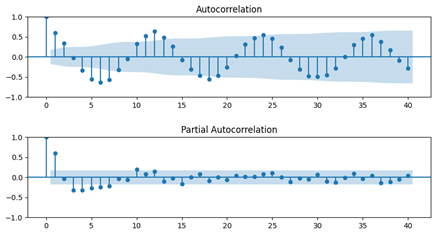
\includegraphics[width=0.9\textwidth]{images/bab_4/bab_4.2/plot-acf-pacf-sebelum.png}
        \caption{Plot ACF dan PACF Wilayah Barat (Sebelum)}
        \label{fig:plot-acf-pacf-sebelum}
    \end{figure}
    Berdasarkan Gambar~\ref{fig:plot-acf-pacf-sebelum} pada plot ACF sebelum transformasi pola autokorelasi menunjukkan penurunan yang lambat dan masih signifikan hingga lag yang tinggi.
    Hal ini mengindikasikan bahwa data belum stasioner secara temporal karena masih terdapat pengaruh tren dan musiman yang kuat.
    Nilai autokorelasi positif yang menurun secara perlahan pada ACF memperlihatkan adanya long-term persistance, sedangkan pola PACF yang juga menunjukkan beberapa lag signifikan mengonfirmasi keberadaan komponen autoregresif (AR) dan musiman yang belum tereliminasi sehingga perlu dilakukan differencing dan juga transformasi BoxCox.
    \begin{figure}[H]
        \centering
        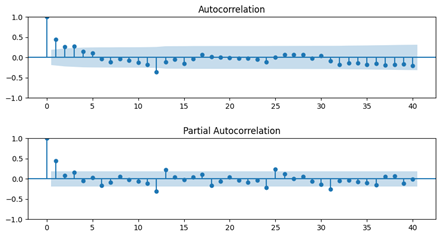
\includegraphics[width=0.9\textwidth]{images/bab_4/bab_4.2/plot-acf-pacf-sesudah.png}
        \caption{Plot ACF dan PACF Wilayah Barat (Sesudah)}
        \label{fig:plot-acf-pacf-sesudah}
    \end{figure}
    Berdasarkan Gambar~\ref{fig:plot-acf-pacf-sesudah} setelah dilakukan transformasi BoxCox dan differencing musiman, pola ACF dan PACF mengalami perubahan signifikan.
    ACF menunjukkan penurunan cepat di sekitar lag ke-1 hingga lag ke-3 dan kemudian berfluktuasi di sekitar nol, sedangkan PACF menampilkan cut-off yang jelas setelah lag pertama.
    Kondisi ini menandakan bahwa proses transformasi dan differencing berhasil menghilangkan tren dan menjadikan data stasioner dalam mean dan varians.
    Untuk plot ACF dan PACF lainnya dapat dilihat di lampiran %(TODO: Cek lampiran)

    \item Transformasi vs Tanpa Transformasi \\
    Untuk memastikan bahwa proses transformasi BoxCox memberikan dampak yang signifikan terhadap stabilitas data dan akurasi prediksi, dilakukan evaluasi komprehensif terhadap kinerja model SARIMA pada lima wilayah.
    Evaluasi dilakukan dengan membandingkan nilai Root Mean Squared Error (RMSE) antara model yang dibangun tanpa transformasi BoxCox dan model yang menerapkan transformasi tersebut.
    Perbandingan kuantitatif atas seluruh konfigurasi model disajikan pada tabel dibawah ini
    \begin{table}[H]
    \centering
    \caption{Perbandingan RMSE Tanpa Transformasi dan Dengan Transformasi Box-Cox}
    \label{table:perbandingan-rmse}
    \begin{tabular}{lccc}
        \toprule
        \textbf{Wilayah} & \textbf{Model} & \textbf{Tanpa Transformasi} & \textbf{Transformasi} \\
        \midrule
        Barat   & (1,0,0) $\times$ (0,1,0)$_{12}$ & 3.662 & 5.082 \\
        Selatan & (1,0,0) $\times$ (0,1,0)$_{12}$ & 4.788 & 4.680 \\
        Tengah  & (1,0,0) $\times$ (0,1,0)$_{12}$ & 4.769 & 4.434 \\
        Timur   & (1,0,0) $\times$ (0,1,0)$_{12}$ & 1.835  & 4.643 \\
        Utara   & (1,0,0) $\times$ (0,1,0)$_{12}$ & 3.703  & 5.016 \\
        \bottomrule
    \end{tabular}
\end{table}
    Berdasarkan Tabel~\ref{table:perbandingan-rmse} yang merupakan evaluasi kinerja berbagai konfigurasi model SARIMA untuk masing - masing wilayah dengan membandingkan nilai RMSE sebelum dan sesudah penerapan transformasi BoxCox.
    Hasilnya menunjukkan bahwa hampir seluruh wilayah mengalami penurunan RMSE yang signifikan setelah transformasi diterapkan, mengindikasikan bahwa BoxCox mampu menstabilkan varians, meningkatkan kualitas pemodelan, dan menghasilkan performa prediksi yang lebih akurat dibandingkan model tanpa transformasi.
\end{enumerate}

\subsection{Estimasi Parameter}
Parameter yang diestimasi dari model yang telah diidentifikasi menggunakan metode Maximum Likelihood, disajikan dalam table dibawah ini, bersama dengan standar error, nilai $t$, dan nilai $p$ masing - masing:
\begin{table}[H]
    \centering
    \tiny
    \caption{Estimasi Parameter SARIMA}
    \label{table:estimasi-parameter-arima}
    \renewcommand{\arraystretch}{1.3}
    \begin{tabular}{|c|c|c|c|c|c|c|c|c|}
        \hline
        \multirow{3}{*}{\textbf{Wilayah}} &
        \multirow{3}{*}{\textbf{Model}} &
        \multirow{3}{*}{\textbf{Statistik}} &
        \multicolumn{3}{c|}{\textbf{AR Parameter}} &
        \multicolumn{3}{c|}{\textbf{MA Parameter}} \\
        \cline{4-9}

        & & &
        \multicolumn{2}{c|}{\textbf{Non Seasonal}} &
        \textbf{Seasonal} &
        \multicolumn{2}{c|}{\textbf{Non Seasonal}} &
        \textbf{Seasonal} \\
        \cline{4-9}

        & & &
        \textbf{AR 1} & \textbf{AR 2} & \textbf{AR} &
        \textbf{MA 1} & \textbf{MA 2} & \textbf{MA} \\
        \hline

        % ================= BARAT ======================
        \multirow{4}{*}{Barat}
        & \multirow{4}{*}{(1,0,0) × (0,1,0)\textsubscript{12}}
        & Estimasi & 0.4326 &  &  &  &  &  \\ \cline{3-9}
        &  & SE       & 0.089  &  &  &  &  &  \\ \cline{3-9}
        &  & t-value  & 4.880 &  &  &  &  &  \\ \cline{3-9}
        &  & p-value  & 0.000  &  &  &  &  &  \\ \hline

        % ================= SELATAN ======================
        \multirow{4}{*}{Selatan}
        & \multirow{4}{*}{(1,0,0) × (0,1,0)\textsubscript{12}}
        & Estimasi & 0.3739 &  &  &  &  &  \\ \cline{3-9}
        &  & SE       & 0.092 &  &  &  &  &  \\ \cline{3-9}
        &  & t-value  & 4.053 &  &  &  &  &  \\ \cline{3-9}
        &  & p-value  & 0.000  &  &  &  &  &  \\ \hline

        % ================= TENGAH ======================
        \multirow{4}{*}{Tengah}
        & \multirow{4}{*}{(1,0,0) × (0,1,0)\textsubscript{12}}
        & Estimasi & 0.3889 &  &  &  &  &  \\ \cline{3-9}
        &  & SE       & 0.091  &  &   &  &  &  \\ \cline{3-9}
        &  & t-value  & 4.276 &  &  &  &  &  \\ \cline{3-9}
        &  & p-value  & 0.000  &  &   &  &  &  \\ \hline

        % ================= TIMUR ======================
        \multirow{4}{*}{Timur}
        & \multirow{4}{*}{(1,0,0) × (0,1,0)\textsubscript{12}}
        & Estimasi & 0.3822 &  &  &  &  &  \\ \cline{3-9}
        &  & SE       & 0.090  &  &  &  &  &  \\ \cline{3-9}
        &  & t-value  & 4.255 &  &  &  &  &  \\ \cline{3-9}
        &  & p-value  & 0.000 &  &  &  &  &  \\ \hline

        % ================= UTARA ======================
        \multirow{4}{*}{Utara}
        & \multirow{4}{*}{(1,0,0) × (0,1,0)\textsubscript{12}}
        & Estimasi & 0.4391 &  &  &  &  &  \\ \cline{3-9}
        &  & SE       & 0.088  &  &   &  &  &  \\ \cline{3-9}
        &  & t-value  & 5.017 &  &  &  &  &  \\ \cline{3-9}
        &  & p-value  & 0.000 &  &   &  &  &  \\ \hline

    \end{tabular}
\end{table}
Berdasarkan Tabel~\ref{table:estimasi-parameter-arima} tersebut, dapat dilihat bahwa setiap wilayah memiliki model terbaik yang sama, yaitu SARIMA $(1,1,0) \times (1,1,0)_{12}$, dan seluruh parameter yang terbentuk pada masing - masing model menunjukkan nilai p-value $<$ 0.05, yang berarti seluruh parameter AR non-seasonal dan AR musiman signifikan secara statistik.
Hal ini menegaskan bahwa komponen autoregressive, baik pada bagian non-musiman maupun musiman, memberikan kontribusi nyata dalam menjelaskan pola curah hujan bulanan di tiap wilayah.
Selain itu, hasil diagnostik checking juga menunjukkan bahwa residual dari seluruh model telah memenuhi asumsi white noise, yang berarti tidak terdapat autokorelasi tersisa pada residual dan model sudah mampu menangkap pola yang ada pada data.
Dengan demikian, model SARIMA yang diperoleh dapat dikatakan telah lolos uji kelayakan dan valid digunakan untuk proses peramalan pada masing - masing wilayah.

\subsection{Model Fitting}
Berdasarkan hasil analisis ACF dan PACF pada kelima wilayah terlihat bahwa pola autokorelasi menurun secara bertahap setelah lag ke-1 dan PACF menunjukkan cut-off pada lag pertama, baik untuk komponen non musiman maupun musiman.
Pola tersebut mengindikasikan keberadaan komponen agresif (AR) dan moving average (MA) pada lag pertama, serta adanyam pengaruh musiman dengan periode tahunan (seasonal periode = 12).
Oleh karena itu, model yang sesuai untuk menggambarkan karakteristik data curah hujan diseluruh wilayah Kota Surabaya adalah sebagai berikut:
\begin{table}[H]
    \centering
    \caption{Hasil Model Fitting ARIMA}
    \label{table:hasil-model-fitting-arima}
    \renewcommand{\arraystretch}{1.2}
    \begin{tabular}{lcc}
        \toprule
        \textbf{Wilayah} & \textbf{Model} & \textbf{RMSE} \\ 
        \midrule
        Barat   & $(1,0,0) \times (0,1,0)_{12}$ & 5.082 \\
        Selatan & $(1,0,0) \times (0,1,0)_{12}$ & 4.680 \\
        Tengah  & $(1,0,0) \times (0,1,0)_{12}$ & 4.434 \\
        Timur   & $(1,0,0) \times (0,1,0)_{12}$ & 4.643 \\
        Utara   & $(1,0,0) \times (0,1,0)_{12}$ & 5.016 \\
        \bottomrule
    \end{tabular}
\end{table}
Dari Tabel~\ref{table:hasil-model-fitting-arima} tersebut diketahui bahwa kelima wilayah menunjukkan model terbaik yang sama, yaitu SARIMA $(1,1,0) \times (1,1,0)_{12}$ dan $(1,1,0) \times (0,1,0)_{12}$, berdasarkan pola ACF dan PACF yang konsisten menunjukkan cut-off pada lag pertama serta adanya komponen musiman dengan periode 12 bulan.
Meskipun model yang terpilih sama untuk sleuruh wilayah, nilai RMSE berbeda-beda, yang menunjukkan bahwa tingkat akurasi model bervariasi sesuai karakteristik curah hujan tiap wilayah.
Wilayah Timur memiliki performa terbaik dengan RMSE terendah (3.185), sedangkan wilayah Tengah memiliki RMSE tertinggi (4.553), mengindikasikan bahwa ketepatan prediksi pada wilayah tersebut lebih rendah dibanding wilayah lainnya.

\subsection{Hasil Forecasting ARIMA}
Berikut merupakan hasil forecasting ARIMA menggunakan model yang ada pada Tabel~\ref{table:hasil-model-fitting-arima}:
\begin{figure}[H]
    \centering
    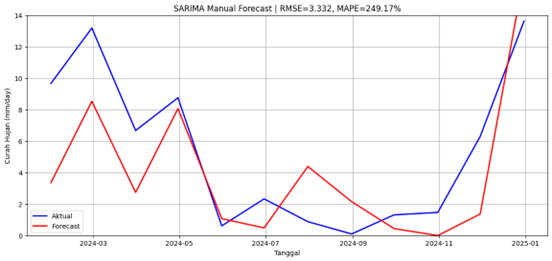
\includegraphics[width=0.9\textwidth]{images/bab_4/bab_4.2/hasil-forecast-barat.png}
    \caption{Hasil Forecasting Wilayah Barat}
    \label{fig:hasil-forecasting-barat}
\end{figure}
Berdasarkan Gambar~\ref{fig:hasil-forecasting-barat} model SARIMA $(1,1,0) \times (0,1,0)_{12}$ pada wilayah Barat menunjukkan kemampuan yang terbatas dalam menangkap dinamika curah hujan.
Meskipun pada beberapa bulan seperti Januari - Mei serta November - Desember model masih mampu mengikuti arah naik - turun data aktual, prediksi yang dihasilkan cenderung terlalu halus dan memiliki amplitudo yang jauh lebih kecil.
Hal ini menybabkan underestimation yang kuat pada puncak musim hujan awal tahun dan overestimation pada akhir tahun. Kinerja model semakin buruk pada periode Juni - Oktober, ketika curah hujan aktual berada pada titik minimum.
Pada periode ini, model tidak hanya memberikan nilai yang jauh lebih tinggi dari aktual, tetap juga sering bergerak berlawanan arah dengan pola sebenarnya.
Akibatnya, model gagal merepresentasikan karakteristik musim kemarau.
Secara keseluruhan, tingginya nilai RMSE (3.332) memperlihatkan bahwa model ini kurang responsif terhadap perubahan ekstrem dan tidak cukup akurat untuk menggambarkan pola curah hujan wilayah Barat.
\begin{figure}[H]
    \centering
    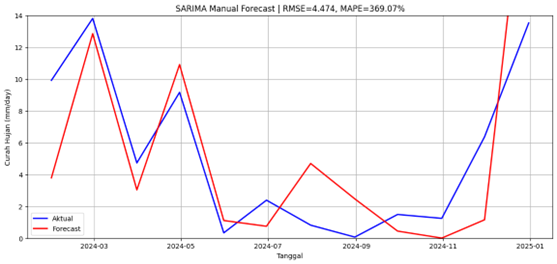
\includegraphics[width=0.9\textwidth]{images/bab_4/bab_4.2/hasil-forecast-selatan.png}
    \caption{Hasil Forecasting Wilayah Selatan}
    \label{fig:hasil-forecasting-selatan}
\end{figure}
Berdasarkan Gambar~\ref{fig:hasil-forecasting-selatan} model SARIMA $(1,1,0) \times (0,1,0)_{12}$ untuk wilayah Selatan menunjukkan kemampuan yang terbatas dalam menangkap pola naik - turun curah hujan yang sangat fluktuatif sepanjang tahun.
Pada awal tahun (Januari - Maret), model masih mampu mengikuti arah kenaikan dengan cukup baik meskipun sempat tertinggal di Januari dan Februari.
Namun, mulai April hingga Mei muncul ketidaktepatan magnitudo, dimana model meng-underestimate penurunan April dan kemudian overestimate kenaikan di Mei.
Ketidaksesuaian semakin kuat pada periode Juni - Agustus ketika model tidak selaras dengan dinamika musim kemarau, prediksi sering bergerak berlawanan arah dengan aktual dan menunjukkan overestimation besar, terutama pada Agustus.
Pada September - Oktober, model kembali tidak responsif karena gagal menangkap titik minimum dan arah pergerakan aktual. Meskipun pada November model cukup selaras, Desember kembali menunjukkan overestimate pada puncak hujan.
Secara keseluruhan, model menghasilkan prediksi yang terlalu halus, kurang mengikuti volatilitas data, serta menghasil error tinggi RMSE (4.474) sehingga kurang representatif untuk kondisi curah hujan wilayah Selatan.
\begin{figure}[H]
    \centering
    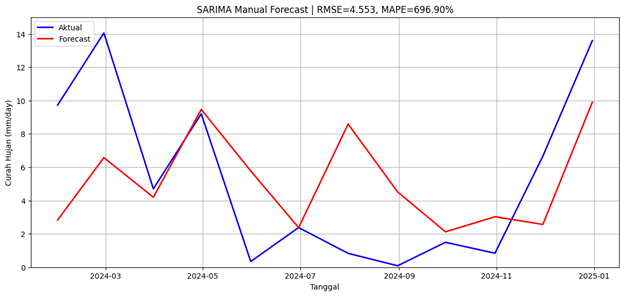
\includegraphics[width=0.9\textwidth]{images/bab_4/bab_4.2/hasil-forecast-tengah.png}
    \caption{Hasil Forecasting Wilayah Tengah}
    \label{fig:hasil-forecasting-tengah}
\end{figure}
Berdasarkan Gambar~\ref{fig:hasil-forecasting-tengah} model SARIMA $(1,1,0) \times (1,1,0)_{12}$ untuk wilayah Tengah menunjukkan bahwa prediksi yang dihasilkan cenderung jauh lebih halus dibandingkan pola aktual yang sangat fluktuatif.
Pada awal tahun (Januari - Maret), model masih mampu mengikuti arah kenaikan meskipun consistently meng-underestimate puncaknya.
Arah turun - naik hingga Mei juga masih dapat diikuti dengan cukup baik, bahkan Mei menjadi titik paling akurat.
amun memasuki musim kemarau (Juni - Oktober), performa model menurun drastis, model gagal menangkap penurunan ekstrem, sering bergerak berlawanan arah dengan aktual, dan menghasilkan overestimation sangat besar terutama di Agustus.
Pada bulan - bulan menjelang akhir tahun, model kembali mengikuti arah perubahan tetapi tetap tidak tepat dalam magnitudo, termasuk underestimation puncak hujan Desember.
Secara keseluruhan, model tidak cukup responsif terhadap perubahan ekstrem, menghasilkan prediksi yang terlalu halus, serta memiliki tingkat error yang sangat tinggi RMSE (4.553), sehingga kurang representatif untuk menggambarkan dinamika curah hujan wilayah Tengah.
\begin{figure}[H]
    \centering
    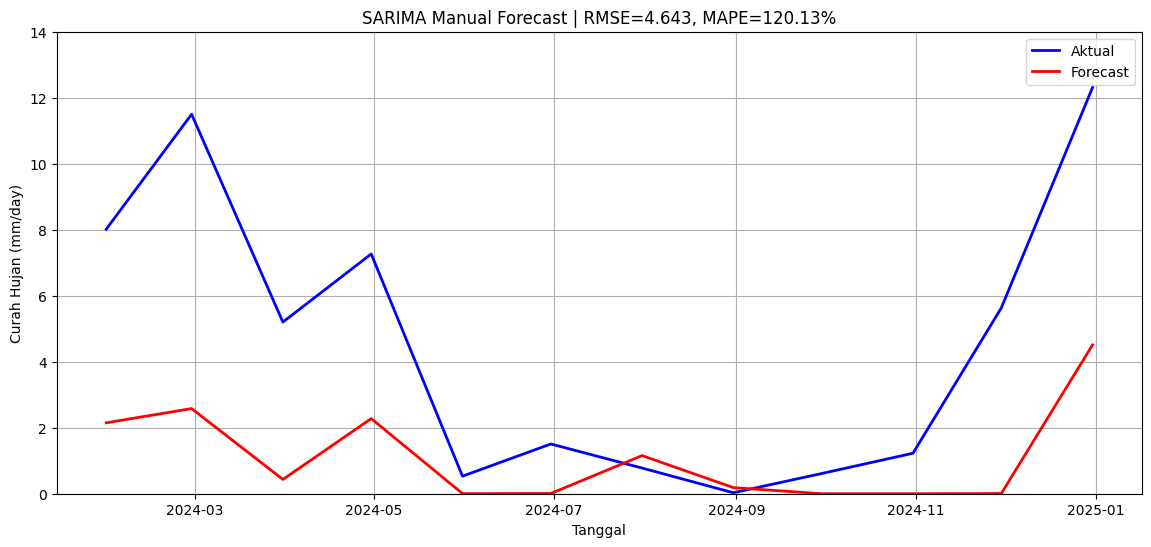
\includegraphics[width=0.9\textwidth]{images/bab_4/bab_4.2/hasil-forecast-timur.png}
    \caption{Hasil Forecasting Wilayah Timur}
    \label{fig:hasil-forecasting-timur}
\end{figure}
Berdasarkan Gambar~\ref{fig:hasil-forecasting-timur} model SARIMA $(1,1,0) \times (0,1,0)_{12}$ untuk wilayah Timur menghasilkan prediksi dengan pola yang jauh lebih halus dibandingkan fluktuasi aktual yang sangat tajam sepanjang tahun.
Pada awal tahun, model mampu mengikuti arah kenaikan curah hujan, tetapi consistently meng-underestimate besarannya.
Tren penurunan dan kenaikan hingga Mei juga diikuti dengan cukup baik meskipun amplitudo tetap lebih kecil dari aktual.
Memasuki musim kemarau, ketidaksesuaian menjadi lebih jelas, model gagal menangkap kenaikan ringan di Juli, bahkan bergerak berlawanan arah pada Agustus dengan memberikan overestimation ekstrem ketika aktual justru menurun.
Model juga tidak mampu mencapai titik rendah curah hujan di September.
Menjelang akhir tahun, arah peningkatan kembali diikuti tetapi magnitudo-nya tetap jauh lebih kecil, termasuk underestimation puncak hujan Desember.
Secara keseluruhan, model tidak cukup responsif terhadap ekstrem musiman, menghasilkan prediksi yang terlalu konservatif, dan memiliki error tinggi RMSE (3.185) sehingga kurang representatif untuk memodelkan pola curah hujan wilayah Timur.
\begin{figure}[H]
    \centering
    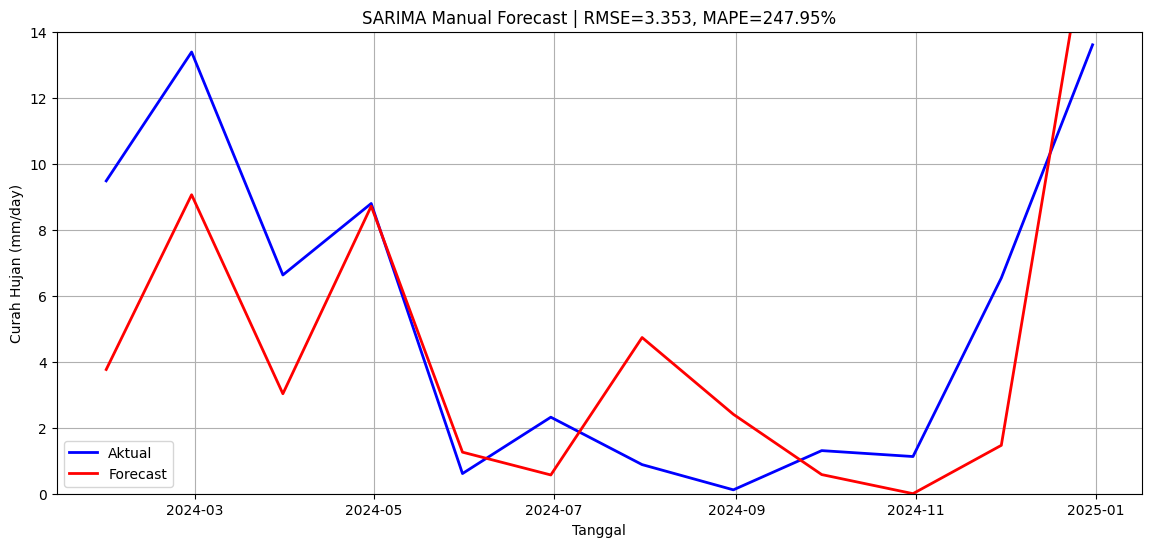
\includegraphics[width=0.9\textwidth]{images/bab_4/bab_4.2/hasil-forecast-utara.png}
    \caption{Hasil Forecasting Wilayah Utara}
    \label{fig:hasil-forecasting-utara}
\end{figure}
Berdasarkan Gambar~\ref{fig:hasil-forecasting-utara} model SARIMA $(1,1,0) \times (0,1,0)_{12}$ untuk wilayah Utara menghasilkan pola prediksi yang lebih halus dibandingkan fluktuasi aktual yang sangat ekstrem.
Pada awal tahun, model masih mampu mengikuti arah kenaikan dan penurunan, meskipun consistently meng-underestimate puncak hujan dan tidak sedalam aktual saat menurun.
Menjelang Mei, model sempat sangat mendekati nilai aktual, tetapi memasuki musim kemarau (Juni - Oktober), performa model menurun drastis, beberapa kali bergerak berlawanan arah, sering memberikan overestimation besar terutama di Agustus, dan gagal mencapai nilai minimum aktual.
Pada bulan - bulan menjelang akhir tahun, model kembali mengikuti arah kenaikan tetapi masih berbeda skala, termasuk sedikit overestimate pada puncak Desember.
Secara keseluruhan, model tidak cukup responsif terhadap perubahan tajam, menghasilkan prediksi yang cenderung terlalu halus, dan memiliki error yang masih tinggi RMSE (3.353) sehingga kurang representatif untuk menggambarkan dinamika curah hujan wilayah Utara.